\section{Introduction}
This chapter will outline the usage of Bre\'guet's range equations in two methods for finding the pareto frontier of optimal range and endurance tradeoffs for an aircraft, given certain parameters. Additionally, a method for determining a tradeoff frontier for endurance of an aircraft's flight and the radius of its loiter. Lastly, the application of this approach will be explained in detail.\par
\section{Current Methodology}
\section{Deriving Bre\'guet Equations}
Two main equations are derived from the general range equation seen in Eq. \ref{eqRangeEq}. The first logically flows from the need to maximize range while assuming a constant thrust specific fuel consumption (constant altitude and throttle setting). Maximizing $V/T_A$ will maximize range and $T \approx T_R = D$ where $D$ is drag. Thus, to maximize range, the aircraft must be flown at $(D/V)_{min}$. The following equivalent equations follow from the assumption that the aircraft will fly at straight, level, unaccelerated flight.
\begin{align}
    T_A&=D = C_Dq_{\infty}S \dfrac{W}{L} = \dfrac{C_Dq_{\infty}S(W)}{C_Lq_{\infty}S} = \dfrac{C_D}{C_L}W\\
    L &= W = C_Lq_{\infty}S = C_L\dfrac{1}{2}\rho_{\infty}V^2_{\infty}S \Rightarrow V_{\infty} = \sqrt{\dfrac{2W}{\rho_{\infty}C_LS}}
    \label{eq: VequivalentEq}
\end{align}
These equations can be used in the general range equation shown in Eq. \ref{eq:genRangeFull}.
\begin{equation}
\label{eq:genRangeFull}
    \begin{aligned}
        R &= \int_{W_f}^{W_i}\sqrt{\dfrac{2W}{\rho_{\infty}C_LS}}\left(\dfrac{1}{TSFC}\right)\left(\dfrac{C_L}{C_D}\right)\left(\dfrac{1}{W}\right)dW\\
        R &= \int_{W_f}^{W_i}\sqrt{\dfrac{2W}{\rho_{\infty}S}}\left(\dfrac{1}{TSFC}\right)\left(\dfrac{C_L^{1/2}}{C_D}\right)\left(\dfrac{1}{W}\right)dW\\
    \end{aligned}
\end{equation}
Further simplifying assumptions are used in general aircraft performance in \cite{IntroACMechanics} to derive the following Bre\'guet range equation in Eq. \ref{eq:LinRangeEq}. These include a constant altitude which implies a constant density, $\rho_{\infty}$, a constant angle of attack which makes $C_L$ and $C_D$ constant, and similar to the general equation, TSFC is constant.
\begin{equation}
\label{eq:LinRangeEq}
    \begin{aligned}
        R &= \sqrt{\dfrac{2}{\rho_{\infty}S}}\left(\dfrac{1}{TSFC}\right)\left(\dfrac{C_L^{1/2}}{C_D}\right)\int_{W_f}^{W_i}\dfrac{dW}{\sqrt{W}}\\
        R &= \sqrt{\dfrac{2}{\rho_{\infty}S}}\left(\dfrac{2}{TSFC}\right)\left(\dfrac{C_L^{1/2}}{C_D}\right)(\sqrt{W_i}-\sqrt{W_f})
    \end{aligned}
\end{equation} \par
In addition to the linear range equation, another simplification of the general range equation involves assuming constant cruise velocity, a constant angle of attack, and a constant thrust specific fuel consumption. This equation is referred to in \cite{IntroACMechanics} as the constant speed cruise range equation. Using the general range equation in \ref{eq:genRangeFull} and substituting $V$ in for the equivalent formula presented in \ref{eq: VequivalentEq}, the following equation is derived.
\begin{equation}
    R = \dfrac{V}{TSFC}\left(\dfrac{C_L}{C_D}\right)\ln{\dfrac{W_i}{W_f}}
\end{equation}
This equation is maximized when $V\dfrac{C_L}{C_D}$ is maximized or equivalently when $\dfrac{C_L^{1/2}}{C_D}$ is maximized.

\section{Extracting Parameters}
Parameters for the flight plan can either be user-defined or be defined to maximize performance for a best case scenario. In the interest of simplicity, the F-15C will be used as a general example for how parameters are extracted for maximizing performance and from the existing NASIC model. Parameters for the F-15C's $C_L\text{ and }C_D$ performance are referenced in Figure \ref{fig:machSpeedByGroup}. Each line in the graph represents a mach number which is formed by the value for each coefficient of lift ($C_L$) and the associated coefficient of drag ($C_D$). These are found from historical flying data for each specific aircraft. From the matrix of these values, the lift over drag and $C_L^{1/2}/C_D$ maximums can be found. Where $C_L^{1/2}/C_D$ is maximized, the respective mach number and $C_L/C_D$ can be pulled into the model as a parameter.\par
An example of drag polar outputs from the existing model are shown in Figure (PLACE) for reference. Using 

\begin{figure}%
    \centering
    \subfloat[Lift versus drag curves for all mach numbers.]{{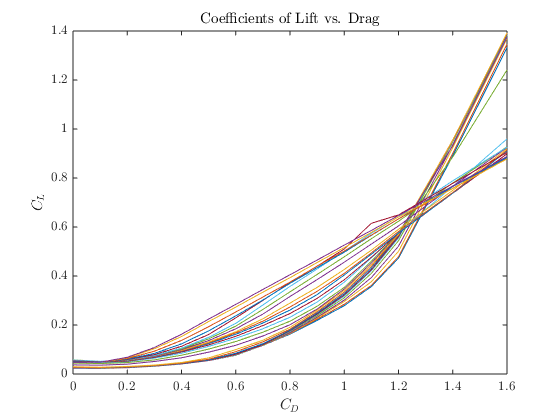
\includegraphics[width=7cm]{Thesis/Method/AllMachNumbers.png} }}%
    \qquad
    \subfloat[Lift versus drag curves defined by mach group.]{{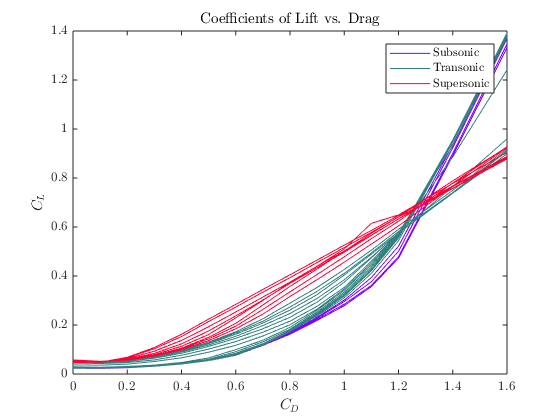
\includegraphics[width=7cm]{Thesis/Method/MachSpeedByGroup.png} }}%
    \caption{Coefficients of lift versus drag for the F-15C.}%
    \label{fig:machSpeedByGroup}%
\end{figure}


